\documentclass[tikz,border=4pt]{standalone}
\usetikzlibrary{positioning,arrows.meta,fit,backgrounds,calc}
\begin{document}
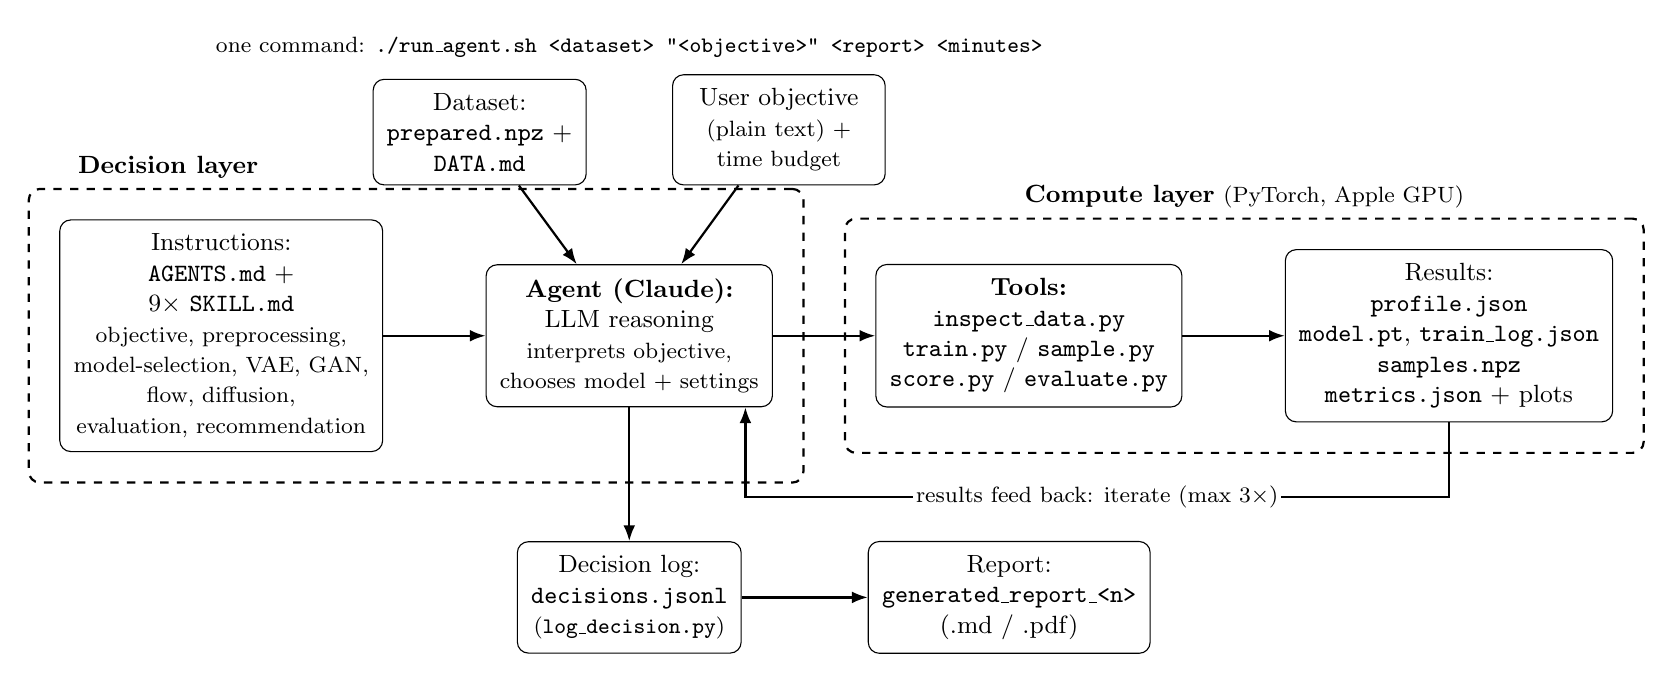
\begin{tikzpicture}[
  node distance=1.1cm and 1.3cm,
  box/.style={draw, rounded corners, align=center, minimum height=1.15cm, minimum width=2.7cm, font=\small, inner sep=5pt},
  arrow/.style={-{Latex[length=2mm]}, thick},
  layer/.style={draw, dashed, rounded corners, thick, inner sep=11pt}
]
\node[box] (agent) {\textbf{Agent (Claude):}\\ LLM reasoning\\ \footnotesize interprets objective,\\ \footnotesize chooses model + settings};
\node[box, above=1.0cm of agent, xshift=-1.9cm] (dataset) {Dataset:\\ \texttt{prepared.npz} +\\ \texttt{DATA.md}};
\node[box, above=1.0cm of agent, xshift=1.9cm] (objective) {User objective\\ \footnotesize (plain text) +\\ \footnotesize time budget};
\node[box, left=of agent] (instructions) {Instructions:\\ \texttt{AGENTS.md} +\\ 9$\times$ \texttt{SKILL.md}\\ \footnotesize objective, preprocessing,\\ \footnotesize model-selection, VAE, GAN,\\ \footnotesize flow, diffusion,\\ \footnotesize evaluation, recommendation};
\node[box, right=of agent, minimum width=3.0cm] (tools) {\textbf{Tools:}\\ \texttt{inspect\_data.py}\\ \texttt{train.py} / \texttt{sample.py}\\ \texttt{score.py} / \texttt{evaluate.py}};
\node[box, right=of tools, minimum width=3.0cm] (results) {Results:\\ \texttt{profile.json}\\ \texttt{model.pt}, \texttt{train\_log.json}\\ \texttt{samples.npz}\\ \texttt{metrics.json} + plots};
\node[box, below=1.7cm of agent] (log) {Decision log:\\ \texttt{decisions.jsonl}\\ \footnotesize (\texttt{log\_decision.py})};
\node[box, right=1.6cm of log, minimum width=3.0cm] (report) {Report:\\ \texttt{generated\_report\_<n>}\\ (.md / .pdf)};
\node[font=\footnotesize, align=center, above=0.15cm of dataset, xshift=1.9cm] (cmd) {one command: \texttt{./run\_agent.sh <dataset> "<objective>" <report> <minutes>}};

\begin{pgfonlayer}{background}
\node[layer, fit=(instructions)(agent), label={[font=\small]above left:\textbf{Decision layer}}] {};
\node[layer, fit=(tools)(results), label={[font=\small]above:\textbf{Compute layer} \footnotesize(PyTorch, Apple GPU)}] {};
\end{pgfonlayer}

\draw[arrow] (dataset) -- (agent);
\draw[arrow] (objective) -- (agent);
\draw[arrow] (instructions) -- (agent);
\draw[arrow] (agent) -- (tools);
\draw[arrow] (tools) -- (results);
\draw[arrow] (agent) -- (log);
\draw[arrow] (log) -- (report);
\draw[arrow] (results.south) -- ++(0,-0.95) -| node[font=\footnotesize, fill=white, inner sep=1pt, pos=0.25] {results feed back: iterate (max 3$\times$)} ($(agent.south east)+(-0.35,0)$);
\end{tikzpicture}
\end{document}
